\chapterimage{orange2.jpg}
\chapterspaceabove{6.75cm} 
\chapterspacebelow{7.25cm} 
\chapter{Boolean Algebra and Further Logic}
    In the first chapter of this book, we discussed the very basic of mathematics, 
    proof and propositions. This chapter aims to excavate mathematical logics in 
    further details. With Boolean Algebra, we can explain more thoroughly on
    the mechanism of logics and mathematical proof, and on top of that, we can 
    figure out how computer functions, as well as how integrated circuits are 
    constructed.
    \section{Boolean Expression and Truth Table}
        We call Boolean Algebra "Algebra" of course, because it possesses property of Algebra.
        We will start with basic algebra operation and thus, proceed to get the rule of 
        Boolean operation, which we call the "Truth Table".
    \subsection{Property of Algebra Operation}
        For normal algebra operation of numbers, we have the following general law
        by representing the number in $x$, $y$, and $z$.
        \begin{table}[ht]
            \label{algelaw}
            \centering
            \caption{Common Algebraic Laws}
            \begin{tabular}{lll}
            \toprule
            \textbf{Law} & \textbf{Addition Expression} & \textbf{Multiplication Expression} \\
            \midrule
            Identity & \( x + 0 = x \) & \( x \cdot 1 = x \) \\
            Property of Zero & & \( x \cdot 0 = 0 \) \\
            Inverse & \( x + (-x) = 0 \) & \( x \cdot x^{-1} = 1 \), for \( x \neq 0 \) \\
            Commutative & \( x + y = y + x \) & \( x \cdot y = y \cdot x \) \\
            Associative & \( (x + y) + z = x + (y + z) \) & \( (x \cdot y) \cdot z = x \cdot (y \cdot z) \) \\
            Distributive & &\( x \cdot (y + z) = x \cdot y + x \cdot z \) \\
            \bottomrule
            \end{tabular}
        \end{table}
        In this case, we call $x$, $y$, and $z$ variables as in programming. for 
        all possible values of these variables, these laws hold.
        Why these laws are important is that all algebra expressions is derived
        from these laws, which means we can prove any equality that is correct.
        We take $-1 \time -1$ as an example. One may say without a second thought that
        the answer is 1. But why? Can we prove it? Now we try to prove it using the
        common algebraic laws.
        \begin{example}
            Prove that $(-1)\times (-1) = 1$
        \end{example}
        \begin{proof}
            \begin{align*}
                 & ( -1) \times ( -1)\\
                = & (( -1) \times ( -1)) +0\ ( Addition\ Identity\ )\\
                = & (( -1) \times ( -1)) +\ (( -1) +1) \ ( Addition\ Inverse)\\
                = & ((( -1) \times ( -1) +( -1)) +1\ ( Associative\ Law\ of\ Addition)\\
                = & ((( -1) \times ( -1) +(( -1) \times 1)) +1\ ( Multiplication\ Identity)\\
                = & (( -1) \times (( -1) +1)) +1\ ( Distributive\ Law)\\
                = & (( -1) \times 0) \ +\ 1\ ( Addition\ Inverse)\\
                = & 0+1\ ( Multiplication\ Property\ of\ Zero)\\
                = & 1+0\ (Commutative\ Law\ of\ Addition)\\
                = & 1\ ( Addition\ Identity)
            \end{align*}
            \begin{remark}
                Some people may not understand why we have to write $0+1$ into $1+0$. This is because
                Addition Identity is only defined in the table as $x+0=x$, so we need to apply Commutative
                law of addition to fit it into the known conclusion.
            \end{remark}
        \end{proof}

        After seeing this, you may think, do we really have to know this to make sure that $-1\times-1=1$?
        Of course not, but keep in mind that \textbf{Every mathematical conclusion cannot be simply referred as
        rules such as "a negative times negative give you a positive number", but by meticulous, reasonable, and 
        replicable proof.}

    \subsection{Boolean Expression and Truth Table}
        Hold on a second, isn't this chapter on Boolean Algebra? Why we still need to go over these
        old knowledge from primary school? Well, this is because we will prove Boolean expression in the
        same way. Before that, we introduce Boolean value and operations. 
        % Definition of Boolean Values
        \begin{definition}[Boolean Values]
        In mathematics and computer science, a Boolean value is defined as an element of the Boolean domain \(B\), which can be mathematically represented as:
        \[
        \B = \{0, 1\}
        \]
        where:
        \begin{itemize}
            \item \(0\) typically represents \textit{false}
            \item \(1\) typically represents \textit{true}
        \end{itemize}
        \end{definition}
        Some may be confused by true and false here. Just recall what we have done to propositions in
        the first chapter in this book. When a statement holds for given condition, we take it as
        correct, while incorrect when it does not hold. Boolean value is the basis of Boolean Expression,
        and \textbf{all valid boolean expression could be reduced or simplified to a Boolean value}.
        % Boolean Operations
        \begin{definition}[Boolean Operations]
        Boolean algebra involves operations such as AND, OR, NOT, XOR, which operate on these Boolean values. These operations are defined as follows:
        \begin{itemize}
            \item \textbf{AND} (\(\land\)): An operation on two Boolean values that returns \textit{true} if both operands are \textit{true}, otherwise returns \textit{false}.
            \item \textbf{OR} (\(\lor\)): An operation on two Boolean values that returns \textit{true} if at least one of the operands is \textit{true}, otherwise returns \textit{false}.
            \item \textbf{NOT} (\(\lnot\)): A unary operation that returns \textit{true} if the operand is \textit{false} and vice versa.
            \item \textbf{XOR} (\(\oplus\)): An operation on two Boolean values that returns \textit{true} if the operands are different, otherwise returns \textit{false}.
        \end{itemize}
        \begin{remark}
            There are more Boolean operators to be discussed later.
        \end{remark}
        \end{definition}
        In computer science, Boolean values are fundamental in conditional statements and loops, where they determine the flow of control in algorithms and programs. They are also essential in the design of electronic circuits and digital computing.
        The following table shows the truth table of these basic Boolean operations. the first column
        shows the combination of inputs for the specific operator, and the second column shows the
        result of operation.
        \begin{table}[ht] \label{truthtab}
            \centering % This centers the entire table construct
            
            \noindent
            \begin{tabular}{c|c}
            \textbf{A} & $\neg \textbf{A}$ \\
            \hline
            F & T \\
            T & F \\
            \end{tabular}
            \quad % Reduce the space between tables
            \begin{tabular}{cc|c}
            \textbf{A} & \textbf{B} & $\textbf{A} \land \textbf{B}$ \\
            \hline
            F & F & F \\
            F & T & F \\
            T & F & F \\
            T & T & T \\
            \end{tabular}
            
            \vspace{2mm} % Reduce the vertical space between the rows of tables
            
            \noindent
            \begin{tabular}{cc|c}
            \textbf{A} & \textbf{B} & $\textbf{A} \lor \textbf{B}$ \\
            \hline
            F & F & F \\
            F & T & T \\
            T & F & T \\
            T & T & T \\
            \end{tabular}
            \quad % Reduce the space between tables
            \begin{tabular}{cc|c}
            \textbf{A} & \textbf{B} & $\textbf{A} \oplus \textbf{B}$ \\
            \hline
            F & F & F \\
            F & T & T \\
            T & F & T \\
            T & T & F \\
            \end{tabular}
            
            \caption{Common Boolean Operators Truth Tables}
        \end{table}

        It's noticeable that different Boolean operators may differ in the number of input. $\lnot$ operator
        takes only one Boolean variable (input) to get an output by negating the input, however the rest 
        take two inputs and produce one output. 
        
        At the beginning of the section, we have defined Boolean
        space $B=\{0,1\}$, but why George Boole(The British mathematician who initiate this idea) define 
        Boolean value with a set containing only zero and one? This is actually because, \textbf{The foundation
        of Boolean Algebra is set upon operations involving 0 and 1}. To explicit, I need to clarify that
        among the four operators introduced above, $\lnot$, $\land$, and $\lor$ are the very basic of all
        Boolean expressions, which means other Boolean operators could be written in an equivalent form with
        these basic operators. For example, we can write XOR($\oplus$) in the other three operators:
        \begin{equation}
            \label{xor}
            A \oplus B= (A \land \lnot B) \lor(\lnot A \land B)
        \end{equation}
        It doesn't really matter if you find the RHS strange,as all we need now is just know the fact 
        that we can write it in this form. We will discuss the expression in details in the next section.
        Now let's refocus on Boolean space \{0,1\}. We all know that there are four basic operations in 
        algebra which are addition, subtraction, multiplication, and division. But generally, we say there 
        are only two basic operations in algebra, which are $+$ and $\times$, as subtraction and division are
        just inverse operation of addition and multiplication. Let's look in to the table of addition and 
        multiplication of 0 and 1 listed below.
        \begin{table}[ht]
            \centering % This centers the entire table construct
            \noindent
            \begin{tabular}{cc|c}
                A & B & $A \times B$ \\
                \hline
                0 & 0 & 0 \\
                0 & 1 & 0 \\
                1 & 0 & 0 \\
                1 & 1 & 1 \\
            \end{tabular}
            \quad
            \begin{tabular}{cc|c}
                A & B & $A + B$ \\
                \hline
                0 & 0 & 0 \\
                0 & 1 & 1 \\
                1 & 0 & 1 \\
                1 & 1 & 1 \\     
            \end{tabular}
        \caption{Addition and Multiplication Rule of 0 and 1}
        \end{table}

        Now you may have realized that this is exactly the truth table for $\land$ and $\lor$, you may
        check table \ref{truthtab}.
    
        \subsection{Boolean Identities}
        Now recall that $A \oplus B= (A \land \lnot B) \lor(\lnot A \land B)$. In this
        expression, we cannot get a direct answer from the RHS by using the truth table of $\lor$. So,
        we need to try harder to get the truth table for the expression as shown in the table below.
        \begin{table}[ht]
            \centering
            \caption{Truth table for \((A \land \neg B) \lor (\neg A \land B)\)}
            \begin{tabular}{cc|c|c|c|c|c}
            \hline
            \( A \) & \( B \) & \( \neg B \) & \( A \land \neg B \) & \( \neg A \) & \( \neg A \land B \) & \( (A \land \neg B) \lor (\neg A \land B) \) \\ \hline
            F & F & T & F & T & F & F \\
            F & T & F & F & T & T & T \\
            T & F & T & T & F & F & T \\
            T & T & F & F & F & F & F \\ \hline
            \end{tabular}
            
        \end{table}

        With this method, we can find truth table for more complex expressions, and some of them
        are categorized as \textbf{Basic Boolean Identities}. The LHS and RHS are could be proven qaual
        by listing truth table respectively.

        \begin{table}[H]
            \centering
            \caption{Basic Boolean Identities}
            \begin{tabular}{lll}
            \toprule
            \textbf{Identity} & \textbf{AND Form} & \textbf{OR Form} \\
            \midrule
            Idempotent Law & \( x \cdot x = x \) & \( x + x = x \) \\
            Identity Law & \( x \cdot 1 = x \) & \( x + 0 = x \) \\
            Domination Law & \( x \cdot 0 = 0 \) & \( x + 1 = 1 \) \\
            Complement Law & \( x \cdot \lnot x = 0 \) & \( x + \lnot x = 1 \) \\
            Double Negation Law & \( \lnot(\lnot x) = x \) & \( \lnot(\lnot x) = x \)\\
            Commutative Law & \( x \cdot y = y \cdot x \) & \( x + y = y + x \) \\
            Associative Law & \( x \cdot (y \cdot z) = (x \cdot y) \cdot z \) & \( x + (y + z) = (x + y) + z \) \\
            Distributive Law & \( x \cdot (y + z) = (x \cdot y) + (x \cdot z) \) & \( x + (y \cdot z) = (x + y) \cdot (x + z) \) \\
            De Morgan's Law & \( \lnot(x + y) = \lnot x \cdot \lnot y \) & \( \lnot(x \cdot y) = \lnot x + \lnot y \) \\
            Absorption Law & \( x \cdot (x + y) = x \) & \( x + (x \cdot y) = x \) \\
            \bottomrule
            \end{tabular}
        \end{table}
        \begin{remark}
            If you are confused by the algebra form of Boolean identities, just take $x$, $y$, $z$ as
            $A$, $B$, and $C$; take 0/1 as F/T; take + as $\lor$, and $\times$ as $\land$.
        \end{remark}
        It is quite important to be familiar with these rules, as they are just as essential as
        the normal algebra laws we've learned before, since we may simplify complex Boolean expressions
        using these rules. Also, the proof of some of these identities using truth table will be 
        added to the problem set for this section. If you remain any doubt or confusion about any laws
        given, just try to get the truth table for the LHS and RHS of the identity, simple as that.

        This is actually not yet a complete table of Boolean Identities, two laws are still missing
        from the table, because they are relevant to secondary operator, one of which is already mentioned($\oplus$).

        With these basic Boolean laws, we can derive more interesting and useful theorems. A commonly used theorem when simplifying
        Boolean expression is concensus (or also called redundancy) theorem.
        \begin{theorem}[Concensus Theorem]
            The Consensus Theorem helps simplifying Boolean expressions by eliminating a redundant term, and like other laws, it has both
            OR and AND form. 
            It states that for any Boolean variables $x$, $y$, and $z$:
            \begin{equation*}
                xy\lor\bar{x}z\lor yz=xy\lor\bar{x}z
            \end{equation*}
            Which is equivalent to
            \begin{equation*}
                (x\lor y)(\bar{x}\lor z)(y\lor z)=(x\lor y)(\bar{x}\lor z)
            \end{equation*}
        \end{theorem}
        \begin{proof}
            $$\begin{aligned}
                xy\lor\bar{x}z\lor yz& =xy\lor\bar{x}z\lor(x\lor\bar{x})yz  \\
                &=xy\lor\bar{x}z\lor xyz\lor\bar{x}yz \\
                &=(xy\lor xyz)\lor(\bar{x}z\lor\bar{x}yz) \\
                &=xy(1\lor z)\lor\bar{x}z(1\lor y) \\
                &=xy\lor\bar{x}z
                \end{aligned}$$
            Or in another notation.
            $$\begin{aligned}
                xy + \overline{x}z + yz &= xy + \overline{x}z + (x + \overline{x})yz \\
                &= xy + \overline{x}z + xyz + \overline{x}yz \\
                &= (xy + xyz) + (\overline{x}z + \overline{x}yz) \\
                &= xy(1 + z) + \overline{x}z(1 + y) \\
                &= xy + \overline{x}z
                \end{aligned}$$
        \end{proof}


        \subsubsection*{Secondary Boolean Operators}
        \begin{definition}[Secondary Boolean Operators]
            Secondary operators are derived from basic operators:
            \begin{itemize}
                \item Material conditional: \( x \rightarrow y = \lnot x \lor y \)
                \item Material biconditional: \( x \leftrightarrow y = (x \land y) \lor (\lnot x \land \lnot y) \)
                \item Exclusive OR (XOR): \( x \oplus y = \lnot(x \leftrightarrow y) = (x \lor y) \land (\lnot x \lor \lnot y) = (x \land \lnot y) \lor (\lnot x \land y) \)
                \end{itemize}
        \end{definition}

        Their truth tables for the secondary operation are below:
        \begin{table}[H]
        \centering
        \begin{tabular}{cc|c|c|c}
        \hline
        \( x \) & \( y \) & \( x \rightarrow y \) & \( x \leftrightarrow y \) & \( x \oplus y \) \\
        \hline
        0 & 0 & 1 & 1 & 0 \\
        1 & 0 & 0 & 0 & 1 \\
        0 & 1 & 1 & 0 & 1 \\
        1 & 1 & 1 & 1 & 0 \\
        \hline
        \end{tabular}
        \caption{Truth values of material conditional, biconditional, and XOR for all possible inputs.}
        \end{table}
        The $\rightarrow$ operation holds that $x \rightarrow x = 1$. This expression means
        that when $x=y$, then $x\rightarrow y$ must be true. The complete form of secondary operators
        and the implication identity will be the last Boolean identity to be covered in this chapter.
        \begin{enumerate}
            \item Material Conditional (\(\rightarrow\)):
            The material conditional \( x \rightarrow y \) is read as "if \( x \) then \( y \)" or "\( x \) implies \( y \)". It represents the logical implication. The truth value of \( x \rightarrow y \) is false only when \( x \) is true and \( y \) is false; in all other cases, it is true. This is a bit counter-intuitive when \( x \) is false because the implication will be true regardless of the value of \( y \). It can be expressed using basic operations as \( \lnot x \lor y \).
            
            \item Material Biconditional (\(\leftrightarrow\)):
            The material biconditional \( x \leftrightarrow y \), also known as logical equivalence, is the operation that is true when \( x \) and \( y \) have the same truth values, and false otherwise. It's often read as " \( x \) if and only if \( y \)". It can be formulated as \( (x \land y) \lor (\lnot x \land \lnot y) \), meaning both \( x \) and \( y \) are true, or both are false.
            
            \item Exclusive OR (XOR):
            The exclusive OR \( x \oplus y \) is true when \( x \) and \( y \) have different truth values — that is, one is true and the other is false. It differs from the regular OR operation in that \( x \oplus y \) is false when both \( x \) and \( y \) are true. It can be represented as \( (x \land \lnot y) \lor (\lnot x \land y) \).
        \end{enumerate}
        
        With these basic identities and operators, we can prove more interesting Boolean theorems.
        Below are more theorems to be proved as example. Maybe you are ready to draw a truth table to prove
        them. However, with these basic Boolean Laws, we actually don't have to do that, but prove it
        by using Algebra techniques.
        \begin{example}
            Prove the following identities using the table given earlier.
        \begin{table}[ht]
            \centering
            \begin{tabular}{ll}
            \toprule
            \textbf{Expression} & \textbf{Name} \\
            \midrule
            \( (x \rightarrow \text{False}) = (\lnot x) \) & $\lnot$ as \(\rightarrow\) \\
            \( (x \rightarrow y) = (\lnot y \rightarrow \lnot x) \) & contrapositive \\
            \( ((x \rightarrow y) \land (x \rightarrow z)) = (x \rightarrow (y \land z)) \) & implication \\
            \( ((x \rightarrow y) \land (\lnot x \rightarrow y)) = y \) & absurdity \\
            \( (x \rightarrow (\lnot x)) = (\lnot x) \) & contradiction \\
            \bottomrule
            \end{tabular}
        \end{table}
        \end{example}

        \begin{proof}
            To prove $\lnot$ as \(\rightarrow\), we just need to use the definition of $
            \rightarrow$.
            $$x\rightarrow\text{ False}= \lnot x \lor False = \lnot x + 0 = \lnot x \ \text{(OR Identity Law)}$$
            
            The contrapositive identity states that \( (x \rightarrow y) \) is logically equivalent to \( (\lnot y \rightarrow \lnot x) \).
            \begin{align*}
            x \rightarrow y &\equiv \lnot x \lor y \\
                &\equiv y \lor \lnot x\ \text{(Commutative Law)}\\
            &\equiv \lnot y \rightarrow \lnot x
            \end{align*}
            \begin{remark}
                This proof shows why proof by contrapositive (mentioned in chapter1) is correct.
            \end{remark}
            The implication identity can be proved by showing that \( (x \rightarrow y) \land (x \rightarrow z) \) is equivalent to \( x \rightarrow (y \land z) \).
            \begin{align*}
            (x \rightarrow y) \land (x \rightarrow z) &\equiv (\lnot x \lor y) \land (\lnot x \lor z) \\
            &\equiv \lnot x \lor (y \land z) \\
            &\equiv x \rightarrow (y \land z)
            \end{align*}

            The absurdity identity states that \( (x \rightarrow y) \land (\lnot x \rightarrow y) \) is equivalent to \( y \).
            \begin{align*}
            (x \rightarrow y) \land (\lnot x \rightarrow y) &\equiv (\lnot x \lor y) \land (x \lor y) \\
            &\equiv y \lor (x \land \lnot x) \\
            &\equiv y \lor \text{False} \\
            &\equiv y
            \end{align*}

            The contradiction identity states that \( x \rightarrow (\lnot x) \) is equivalent to \( \lnot x \).
            \begin{align*}
            x \rightarrow (\lnot x) &\equiv \lnot x \lor (\lnot x) \\
            &\equiv \lnot x
            \end{align*}
        \end{proof}
        \begin{remark}
            Some may feel confused by the notation of Boolean expression we use in this chapter.
            Sometimes we use logic notation, while sometimes use algebra operation. Both are ok,
            it's really up to your preference.
        \end{remark}
        When you look through the whole process, you'll find that we are actually doing the same
        thing as simplifying Boolean expressions, where all the laws could be used so that we don't
        need to draw truth table again and again.

        




        \subsection{Exercises}
        \begin{exercise}
            Use table \ref{algelaw} and $1+1=2$ to show that $(x+x)=(2\times x)$.
        \end{exercise}
        \begin{proof}
            \begin{align*}
                ( 2\times x) & =( 1+1) \times x\ ( by\ 1+1=2)\\
                & =\ 1\times x+1\times x\ ( Distributive\ Law)\\
                & =x+x\ ( Multiplication\ Identity)
            \end{align*}
        \end{proof}
        \begin{exercise}
            Show that $((-1)\times x)+x=0$ using the table.
        \end{exercise}
        \begin{proof}
            \begin{align*}
                (( -1) \times x) +x & =x( -1+1) \ ( Distributive\ Law)\\
                 & =\ x\times 0\ ( Addition\ Inverse)\\
                 & =0\ ( Multiplication\ Property\ of\ Zero)
            \end{align*}
        \end{proof}
        \begin{exercise}
            Show that $(x+(((-1)\times (x+y))+z)) + y =z$, you may use the conclusion of previous
            exercise.
        \end{exercise}
        \begin{proof} 
            To make it clear, we use square and curly bracket for different layers of parenthesis.
            \begin{align*}
                \  & \{x+[((-1) \times ( x+y)) +z]\} +y\\
                & =\{x+[(( -1) \times x) +(( -1) \times y)] +z\} +y\ ( Distributive\ Law\ )\\
                & =\{x+(( -1) \times x) +[(( -1) \times y) +z]\} +y\ ( Associative\ Law\ of\ Addition)\\
                & =\{(( -1) \times x) +x+\ [(( -1) \times y) +z]\} +y( Commutative\ Law\ of\ Addition)\\
                & =0+\{[(( -1) \times y) +z] +y\}\ ( Previous\ Conclusion)\\
                & =\{[(( -1) \times y) +z] +y\} +0\ ( Commutative\ Law\ of\ Addition)\\
                & =\{[(( -1) \times y) +z] +y\} \ ( Addition\ Identity)\\
                & =(( -1) \times y) +( z+y) \ ( Associative\ Law\ of\ Addition)\\
                & =( z+y) +(( -1) \times y) \ ( Commutative\ Law\ of\ Addition)\\
                & =z+[ y+(( -1) \times y)] \ ( Associative\ Law\ of\ Addition)\\
                & =z+[(( -1) \times y) +y] \ ( Commutative\ Law\ of\ Addition)\\
                & =z+0\ ( Previous\ Conclusion)\\
                & =z\ ( Addition\ Identity)
            \end{align*}
            
        \end{proof}
        
        \begin{exercise}
            Use truth table to show that De Morgan's Law is correct.
        \end{exercise}
        \begin{proof}
            De Morgan's First Law: \( \lnot (A \land B) = \lnot A \lor \lnot B \)
            
            \begin{tabular}{cc|c|c|c}
            \toprule
            \( A \) & \( B \) & \( A \land B \) & \( \lnot (A \land B) \) & \( \lnot A \lor \lnot B \) \\
            \midrule
            0 & 0 & 0 & 1 & 1 \\
            0 & 1 & 0 & 1 & 1 \\
            1 & 0 & 0 & 1 & 1 \\
            1 & 1 & 1 & 0 & 0 \\
            \bottomrule
            \end{tabular}

            \vspace{2em} 

            De Morgan's Second Law: \( \lnot (A \lor B) = \lnot A \land \lnot B \)

            \begin{tabular}{cc|c|c|c}
            \toprule
            \( A \) & \( B \) & \( A \lor B \) & \( \lnot (A \lor B) \) & \( \lnot A \land \lnot B \) \\
            \midrule
            0 & 0 & 0 & 1 & 1 \\
            0 & 1 & 1 & 0 & 0 \\
            1 & 0 & 1 & 0 & 0 \\
            1 & 1 & 1 & 0 & 0 \\
            \bottomrule
            \end{tabular}
        \end{proof}

        \begin{exercise}
            Use truth table to show that Absorption Law is correct.
        \end{exercise}
        \begin{proof}
            \begin{tabular}{cc|c|c}
                \hline
                \( x \) & \( y \) & $x \lor y$&\( x \land (x \lor y) \) \\
                \hline
                T & T & T & T \\
                T & F & T & T \\
                F & T & F & F \\
                F & F & F & F \\
                \hline
            \end{tabular}
            \quad
            \begin{tabular}{cc|c|c}
                \hline
                \( x \) & \( y \)&$x \land y$ & \( x \lor (x \land y) \) \\
                \hline
                T & T& T& T \\
                T & F& F& T \\
                F & T& F& F \\
                F & F& F& F \\
                \hline
            \end{tabular}
        \end{proof}

        \begin{exercise}
            Show the truth table of $\displaystyle x\lor (( \lnot y) \land ( \lnot z))$.
        \end{exercise}
        \textbf{Hint:} For Boolean expression of 3 variable, there will be more combinations.
        
        \textbf{Solution:}

        \begin{table}[ht]
            \centering
            \caption{Truth table for the expression \( x \lor ((\lnot y) \land (\lnot z)) \)}
            \begin{tabular}{ccc|c|c|c|c}
            \hline
            \( x \) & \( y \) & \( z \) & \( \lnot y \) & \( \lnot z \)& $(\lnot y) \land (\lnot z)$ & \( x \lor ((\lnot y) \land (\lnot z)) \) \\
            \hline
            0 & 0 & 0 & 1 & 1 &1& 1 \\
            0 & 0 & 1 & 1 & 0 &0& 0 \\
            0 & 1 & 0 & 0 & 1 &0& 0 \\
            0 & 1 & 1 & 0 & 0 &0& 0 \\
            1 & 0 & 0 & 1 & 1 &0& 1 \\
            1 & 0 & 1 & 1 & 0 &0& 1 \\
            1 & 1 & 0 & 0 & 1 &0& 1 \\
            1 & 1 & 1 & 0 & 0 &0& 1 \\
            \hline
            \end{tabular}
 
        \end{table}

        \begin{exercise}
            Given the expressions:
            \begin{align*}
            1. & \quad (x \rightarrow y) \land (\lnot x \rightarrow \lnot y) \\
            2. & \quad ((\lnot x) \lor y) \land (x \lor (\lnot y)) \\
            3. & \quad \lnot((x \land (\lnot y)) \lor ((\lnot x) \land y)) \\
            4. & \quad \lnot((x \lor y) \land (\lnot x \lor \lnot y)) \\
            \end{align*}
            Show that they are equivalent and find the common (simplified) form of the four expression
        \end{exercise}
        \begin{proof}
            \begin{align*}
                (x \rightarrow y) \land (\neg x \rightarrow \neg y) & \equiv (\neg x \lor y) \land (x \lor \neg y) && \text{(Implication equivalence)} \\
                & \equiv (x \lor \neg y) \land (\neg x \lor y) && \text{(Commutativity of OR)} \\
                & \equiv (x \lor \neg y) \land (y \lor \neg x) && \text{(Commutativity of AND)}
                \end{align*}

                \begin{align*}
                    ((\neg x) \lor y) \land (x \lor (\neg y)) & \equiv (y \lor \neg x) \land (x \lor \neg y) && \text{(Commutativity of OR)} \\
                    & \equiv (x \lor \neg y) \land (y \lor \neg x) && \text{(Commutativity of AND)}
                    \end{align*}
            
                    \begin{align*}
                        \neg((x \land (\neg y)) \lor ((\neg x) \land y)) & \equiv \neg(x \land (\neg y)) \land \neg((\neg x) \land y) && \text{(De Morgan's laws)} \\
                        & \equiv (\neg x \lor y) \land (x \lor \neg y) && \text{(De Morgan's laws)} \\
                        & \equiv (x \lor \neg y) \land (y \lor \neg x) && \text{(Commutativity of OR and AND)}
                        \end{align*}

                        \begin{align*}
                            \neg((x \lor y) \land (\neg x \lor \neg y)) & \equiv \neg(x \lor y) \lor \neg(\neg x \lor \neg y) && \text{(De Morgan's laws)} \\
                            & \equiv (\neg x \land \neg y) \lor (x \land y) && \text{(De Morgan's laws)} \\
                            & \equiv (x \land y) \lor (\neg x \land \neg y) && \text{(Commutativity of OR)} \\
                            & \equiv (x \lor \neg y) \land (y \lor \neg x) && \text{(Distribution)}
                            \end{align*}
                            

            These expressions could be simplified to $(\lnot y \lor x)\land(\lnot x\lor y)$, or
            $(y\rightarrow x)\land(x\rightarrow y)$, which can also be understood as $x$ and $y$
            cannot be true of false in the same time.
        \end{proof}

        \begin{exercise}
            Show that the concensus theorem's two forms are equivalent.
                $$xy\lor\bar{x}z\lor yz=xy\lor\bar{x}z$$
            and
                $$(x\lor y)(\bar{x}\lor z)(y\lor z)=(x\lor y)(\bar{x}\lor z)$$
            are equivalent.
        \end{exercise}
        \textbf{Solution:}
        We can simplify the product form to the standard form easily.
        \begin{align*}
            (x \lor y)(\overline{x} \lor z)(y \lor z) &= x\overline{x} \lor xz \lor y\overline{x} \lor yz \lor xy \lor xz \lor y^2 \lor yz \\
            &= 0 \lor xz \lor y\overline{x} \lor yz \lor xy \lor xz \lor y \lor yz \\
            &= xz \lor y\overline{x} \lor yz \lor xy \\
            &= xy \lor xz \lor y\overline{x}
        \end{align*}

    \section{Boolean Function}
    This section will bring you some further ideas of Boolean operation. Just like we can take a normal algebra
    expression, such as $2x+3$, as a function $f(x)=2x+3$; we can define \textbf{Boolean Function}
    with Boolean operation.
    \begin{definition}[Boolean Function]
    A Boolean function is a function that returns a Boolean value (true or false) for each possible combination of Boolean inputs. 
    $f: B^n \rightarrow B$ is a function from the set of  $n$-tuples of Boolean values to the set of Boolean values, where  $B = \{0, 1\}$.
    \end{definition} 
    For example, we can write the basic operations we just went over in Boolean Functions:
    \begin{enumerate}
        \item Algebraic notation:
        \begin{itemize}
            \item AND: $f(x, y) = x \cdot y$ or $f(x, y) = xy$
            \item OR: $f(x, y) = x + y$
            \item NOT: $f(x) = x'$ or $f(x) = \overline{x}$
        \end{itemize}
        
        \item Logical notation:
        \begin{itemize}
            \item AND: $f(x, y) = x \wedge y$
            \item OR: $f(x, y) = x \vee y$
            \item NOT: $f(x) = \neg x$
        \end{itemize}
    \end{enumerate}

    We have actually learned about this earlier in the chapter. Think about what we have done using truth tables. Just like what you have done at the beginning of 
    learning functions, you were making tables to show all results of each input with their output. For Preliminary functions, we always have 
    $f: R\rightarrow R$, which makes the mapping hard to make table, because there are infinite many real numbers. But things is much easier for Boolean function,
    because we have known in the definition that each function generate only one single output, and the most important part is that we always have limited inputs.
    Since $|B|=2$ for the Boolean Domain, so each input gives us 2 choices only, and therefore when we have $n$ inputs, we have $2^n$ cases only. $2^n$ seems huge,
    but in most cases we have less than 5 inputs in a Boolean function, so the size of the table is still manageable.

    \subsection{Representation of Boolean Function}
    In most cases, we construct a Boolean Function from a given truth table. All Boolean functions could be represented in both
    Disjunctive Normal Form (also known as sum of product;SOP form) and Conjunctive Normal Form (also known as Product of Sum;POS form).
    \begin{definition}[SOP Form]
        The Sum of Products (SOP) form, also known as the Disjunctive Normal Form (DNF), is a way to represent a Boolean function as a sum (logical OR) of product (logical AND) terms. Each product term consists of literals (variables or their complements) that correspond to the function's minterms, which are the input combinations that result in a function value of 1.
        The general form of an SOP expression is:
        \[f(x_1, x_2, \ldots, x_n) = \sum_{i=1}^{m} \prod_{j=1}^{n} x_j^{(i)},\]
        where $m$ is the number of minterms, $n$ is the number of variables, and $x_j^{(i)}$ is either $x_j$ or $x_j'$ (complement of $x_j$) depending on the value of $x_j$ in the $i$-th minterm.
    \end{definition}

    \begin{definition}[POS Form]
        The Product of Sums (POS) form, also known as the Conjunctive Normal Form (CNF), is a way to represent a Boolean function as a product (logical AND) of sum (logical OR) terms. Each sum term consists of literals (variables or their complements) that correspond to the function's maxterms, which are the input combinations that result in a function value of 0.
        The general form of a POS expression is:
        \[f(x_1, x_2, \ldots, x_n) = \prod_{i=1}^{M} \sum_{j=1}^{n} x_j^{(i)},\]
        where $M$ is the number of maxterms, $n$ is the number of variables, and $x_j^{(i)}$ is either $x_j$ or $x_j'$ (complement of $x_j$) depending on the value of $x_j$ in the $i$-th maxterm.
        \end{definition}
    \begin{remark}
        Minterms and maxterms are fundamental building blocks for representing Boolean functions, corresponding to the input combinations that result in function values of 1 and 0, respectively.
    \end{remark}

    But why we are so obsessed with whether the output for one single row is 1(T) or 0 (F)?
    This is because, when we are constructing a Boolean function, we are trying to make the mapping
    from $B^n$ to $B$, while $B = {0,1}$. Hence, we could conclude that the result of boolean function
    is actually binary, meaning only two cases for the output(we will talk about it later in the chapter).   
    So, we only need to figure out either of all the cases where the output is 0, or all the cases where the 
    output  is 1. This actually explains what are stated in the \textbf{Canonical Form Theorem}.
    \begin{theorem}[Canonical Form Theorem]
        Any Boolean function can be expressed in either of two canonical forms:
        \begin{enumerate}
        \item Sum of Products (SOP) form, also known as the Disjunctive Normal Form (DNF): Any Boolean function can be represented as a disjunction (OR) of one or more minterms, where a minterm is a product (AND) of literals corresponding to the rows in the truth table where the function value is 1.
        \item Product of Sums (POS) form, also known as the Conjunctive Normal Form (CNF): Any Boolean function can be represented as a conjunction (AND) of one or more maxterms, where a maxterm is a sum (OR) of literals corresponding to the rows in the truth table where the function value is 0.
        \end{enumerate}
        \end{theorem}
        
        \begin{proof}
        To prove the Canonical Form Theorem, we will consider an arbitrary Boolean function $f(x_1, x_2, \ldots, x_n)$ and show that it can be expressed in both SOP and POS forms.
        
        \textbf{Proof of SOP form (DNF):}
        \begin{enumerate}
        \item For each row in the truth table where the function value is 1, create a minterm by taking the conjunction (AND) of the literals corresponding to the input values in that row. If the input variable is 1, use the original variable; if the input variable is 0, use the complement of the variable.
        \item Take the disjunction (OR) of all the minterms obtained in step 1. This resulting expression is the SOP form of the Boolean function.
        \end{enumerate}
        
        Since every row where the function value is 1 is represented by a minterm, and the disjunction of these minterms covers all the cases where the function is 1, the resulting SOP form is equivalent to the original Boolean function.
        
        \textbf{Proof of POS form (CNF):}
        \begin{enumerate}
        \item For each row in the truth table where the function value is 0, create a maxterm by taking the disjunction (OR) of the literals corresponding to the input values in that row. If the input variable is 0, use the original variable; if the input variable is 1, use the complement of the variable.
        \item Take the conjunction (AND) of all the maxterms obtained in step 1. This resulting expression is the POS form of the Boolean function.
        \end{enumerate}
        
        Since every row where the function value is 0 is represented by a maxterm, and the conjunction of these maxterms covers all the cases where the function is 0, the resulting POS form is equivalent to the original Boolean function.
        
        Therefore, any Boolean function can be expressed in either SOP or POS form, proving the Canonical Form Theorem.
        \end{proof}
    \begin{example}
        Considering
        \begin{tabular}{|c|c|c|}
            \hline
            x & y & f(x, y) \\
            \hline
            0 & 0 & 1 \\
            \hline
            0 & 1 & 0 \\
            \hline
            1 & 0 & 0 \\
            \hline
            1 & 1 & 1 \\
            \hline
            \end{tabular}
            .If you are familiar with the Boolean operations, you may have realized this is actually a XNOR operation, which negates XOR.
            We will try to get the Algebra expression of this function in both POS and SOP.
             
    \end{example}
    \begin{solution}
                For the SOP form:
                \begin{itemize}
                    \item Function value is 1 for the corresponding input combinations.
                    \item Smallest terms: $m_0 = x'y'$, $m_3 = xy$.
                    \item SOP form of the Boolean function: $f(x, y) = m_0 + m_3 = x'y' + xy$.
                \end{itemize}
            
                For the POS form:
                \begin{itemize}
                    \item Function value is 0 for the corresponding input combinations.
                    \item Largest terms: $M_1 = x + y'$, $M_2 = x' + y$.
                    \item POS form of the Boolean function: $f(x, y) = M_1 \cdot M_2 = (x + y')(x' + y)$.
                \end{itemize}
                
             These two forms can be converted to each other based on the truth table of a Boolean function.
            \end{solution}

    This method also works for Boolean functions with more variables, and the only difference is that it may take a little more time.
    You may check more relevant problems in the exercises.
    
    \subsection{Properties of Boolean Function}
    In this part of the chapter, we will look into further details of Boolean Expression, specifically, Boolean Function. As an intro, we start with completeness
    and duality of Boolean Function. After this, we will introduce the Fundamental Theorem of Boolean Algebra, also known as Boole's expansion theorem (or Shannon expansion), 
    which in the foundation of logic circuit design and implementation.
    \begin{theorem}[Completeness of Boolean Function]
        A set of Boolean operators is said to be \textit{functionally complete} if every Boolean function can be expressed using only those operators. The following sets are known to be functionally complete:

        \begin{enumerate}
            \item The set \{AND, OR, NOT\}, also known as the standard or canonical basis.
            \item The set \{NAND\}, known as the NAND-only implementation.
            \item The set \{NOR\}, known as the NOR-only implementation.
        \end{enumerate}

        The completeness property is important in digital logic design, as it allows designers to create any desired Boolean function using a minimal set of logic gates.
    \end{theorem}

    \begin{remark}
        If you are getting confused by the word "Logic Gate", just take it as another way we call Boolean or Logic Operators. Logic gates are what electric engineers use
        to construct Boolean circuits, which is not discussed in details in this book, since we only discuss the mathematical aspect of this practice. You may refer
        to \href{https://www.wikiwand.com/en/Logic_gate}{this link}
        if you want to get more details. 
    \end{remark}
    To further illustrate, we could say that all Boolean Functions, or Boolean expressions can be expressed by either combinations of \{AND, OR, NOT\}, or NAND gates(s), or NOR gate(s).
    The first point is already quite clear, we have shown that all secondary operators can be written equivalently in basic operators, \{AND, OR, NOT\}. While NAND and NOR are general 
    logic gates that could construct any logic gates. Below is a simplified proof.
    \begin{proof}
        We start the proof with the fact that all Boolean operations can be written by $\lnot, \land, \lor$ operators.
        To show that all Boolean operations could be implemented by NAND and NOR gate, we only need to show that \{AND, OR, NOT\} can be expressed by both NAND and NOR operator.
        \begin{enumerate}
            \item Using NAND gates:
            \begin{itemize}
                \item NOT gate: A NAND gate with its inputs connected together acts as a NOT gate.
                \item AND gate: A NAND gate with its output inverted by a NOT gate (another NAND gate) acts as an AND gate.
                \item OR gate: An OR gate can be constructed using NAND gates and De Morgan's Law: $x + y = (x' \cdot y')'$.
            \end{itemize}
        
            \item Using NOR gates:
            \begin{itemize}
                \item NOT gate: A NOR gate with its inputs connected together acts as a NOT gate.
                \item OR gate: A NOR gate with its output inverted by a NOT gate (another NOR gate) acts as an OR gate.
                \item AND gate: An AND gate can be constructed using NOR gates and De Morgan's Law: $x \cdot y = (x' + y')'$.
            \end{itemize}
        \end{enumerate}
    Now, we have shown that all the three basic logic gates could be expressed by only NAND and NOR gate(s), which completes the proof.
    \end{proof}
    \begin{remark}
        You can get more details of the logic gates \href{https://www.wikiwand.com/simple/Logic_gate}{here}. This fact is more used in engineering practice but not in mathematics. So you
        just need to know the basic idea (in this book).
    \end{remark}

    \begin{theorem}[Duality of Boolean Function]  
        The duality principle states that for every Boolean function $f(x_1, x_2, \ldots, x_n)$, there exists a dual function $f^D(x_1, x_2, \ldots, x_n)$ that can be obtained by:
        \begin{enumerate}
            \item Replacing every occurrence of 0 with 1 and vice versa.
            \item Replacing every occurrence of AND ($\cdot$) with OR ($+$) and vice versa.
        \end{enumerate}
        Important properties related to duality include:
        \begin{enumerate}
            \item Double duality: $(f^D)^D = f$.
            \item De Morgan's Laws:
            \begin{itemize}
                \item $(x + y)^D = x^D \cdot y^D$
                \item $(x \cdot y)^D = x^D + y^D$
            \end{itemize}
        \end{enumerate}

        The duality principle also holds for other pairs of dual operators, such as NAND and NOR, or implication and converse implication.
    \end{theorem}    
    
    \begin{example}[Duality in Boolean Function]
        Here are some examples:
        \begin{enumerate}
            \item Consider the Boolean function $f(x, y) = x + y'$.
            To find the dual of this function, we follow the steps:
            \begin{enumerate}
                \item Replace every occurrence of 0 with 1 and vice versa.
                \item Replace every occurrence of AND ($\cdot$) with OR ($+$) and vice versa.
            \end{enumerate}
            
            Applying these steps to $f(x, y)$, we get:
            $f^D(x, y) = x' \cdot y$
            
            \item Consider the Boolean function $g(a, b, c) = (a + b) \cdot c'$.
            
            To find the dual of this function, we apply the same steps:
            
            $g^D(a, b, c) = (a' \cdot b') + c$
            
            \item Demonstrating double duality:
            
            Let's take the function $f(x, y) = x + y'$ from Example 1 and find the dual of its dual.
            
            $f(x, y) = x + y'$
            $f^D(x, y) = x' \cdot y$
            
            Now, let's find the dual of $f^D(x, y)$:
            $(f^D)^D(x, y) = (x')' + y' = x + y'$
            
            As we can see, $(f^D)^D(x, y) = f(x, y)$, demonstrating the property of double duality.
        \end{enumerate}
    \end{example}
    
    To explain this further, we can just take it as that for each and every Boolean expression, there is only one specific dual to be obtained by negate each T(1) and F(0)
    and inverse each $\land$ and $\lor$. We can actually find a base case for this. We know that T and F are negation to each other, so we say that T and F are dual
    to one another. With this, we can prove the duality of Boolean Function by MI.

    \begin{proof}
        Let $x_1, x_2, \ldots, x_n$ be Boolean variables. We will prove that for any Boolean function $f(x_1, x_2, \ldots, x_n)$, its dual function $f^D(x_1, x_2, \ldots, x_n)$ satisfies:

        \[f^D(x_1, x_2, \ldots, x_n) = (f(x_1', x_2', \ldots, x_n'))'\]

        \textbf{Base case:} Prove that the duality principle holds for the simplest Boolean functions (i.e., single variables and constants).
        \begin{itemize}
            \item For a single variable $x$, we have $x^D = x'$ and $(x')^D = x$.
            \item For constants 0 and 1, we have $0^D = 1$ and $1^D = 0$.
        \end{itemize}

        \textbf{Inductive step:} Assume that the duality principle holds for Boolean functions $f(x_1, x_2, \ldots, x_n)$ and $g(x_1, x_2, \ldots, x_n)$, i.e., $f^D(x_1, x_2, \ldots, x_n) = (f(x_1', x_2', \ldots, x_n'))'$ and $g^D(x_1, x_2, \ldots, x_n) = (g(x_1', x_2', \ldots, x_n'))'$. Prove that the duality principle also holds for more complex Boolean functions composed of $f$ and $g$.

        For the AND operation:
        \begin{align*}
        (f \cdot g)^D &= f^D + g^D = (f(x_1', x_2', \ldots, x_n'))' + (g(x_1', x_2', \ldots, x_n'))' \\
        &= ((f(x_1', x_2', \ldots, x_n')) \cdot (g(x_1', x_2', \ldots, x_n')))' \\
        &= (f \cdot g)(x_1', x_2', \ldots, x_n')'
        \end{align*}

        For the OR operation:
        \begin{align*}
        (f + g)^D &= f^D \cdot g^D = (f(x_1', x_2', \ldots, x_n'))' \cdot (g(x_1', x_2', \ldots, x_n'))' \\
        &= ((f(x_1', x_2', \ldots, x_n')) + (g(x_1', x_2', \ldots, x_n')))' \\
        &= (f + g)(x_1', x_2', \ldots, x_n')'
        \end{align*}

        \textbf{Induction principle:} Since the duality principle holds for the simplest Boolean functions, and if the duality principle holds for $f$ and $g$, it also holds for more complex Boolean functions composed of $f$ and $g$, we can conclude that the duality principle holds for all Boolean functions.

        This proof uses the basic properties of Boolean algebra, such as double negation ($x'' = x$) and De Morgan's laws. By applying mathematical induction, we start with the simplest Boolean functions and gradually extend the proof to more complex Boolean functions, ultimately proving that the duality principle holds for all Boolean functions.
    \end{proof}
    The proof can also be done using Boolean Algebra Laws, which will be one of the exercises.

    Another important property, or theorem in Boolean Function related to its duality, is Boole's expansion theorem, or also known as Shannon's expansion theorem.
    Shannon's expansion theorem, proposed by the American mathematician Claude Shannon, is a fundamental result in Boolean algebra and switching theory. 
    It provides a systematic method to decompose a Boolean function into simpler subfunctions based on the values of a selected variable. 
    This theorem plays a crucial role in the analysis, synthesis, and minimization of Boolean functions, which are essential in digital logic design, computer 
    science, and various other fields involving logical operations.

    \begin{theorem}[Boole's expansion theorem]
        Boole's expansion theorem, often referred to as the Shannon expansion or decomposition, is the identity: $F=x\cdot\dot{F}_x+x^{\prime}\cdot F_{x^{\prime}}$,where $F$ is any Boolean function, $x$ is a variable, $x^{\prime}$ is the complement of $x$, and $F_x$ and $F_{x^{\prime}}$ are $F$
        with the argument $x$ set equal to 1 and to 0 respectively.
        The terms $F_x$ and $F_{x^{\prime}}$ are sometimes called the positive and negative Shannon cofactors, respectively, of $F$ with respect to
        $x$. These are functions, computed by restrict operator, restrict$(F,x,0)$ and restrict$(F,x,1)$. The former represents  the function $F$ where the variable $x$  
        is set to 0, and the latter represents the restriction of the function $F$ where the variable $x$ is set to 1.
        $$\begin{aligned}&\text{A more explicit way of stating the theorem is:}\\&f(X_1,X_2,\ldots,X_n)=X_1\cdot f(1,X_2,\ldots,X_n)+X_1^{\prime}\cdot f(0,X_2,\ldots,X_n)\end{aligned}$$
    \end{theorem}
    \begin{proof}[Proof of Shannon's Expansion Theorem]
        Let $f(x_1, x_2, \ldots, x_n)$ be a Boolean function of $n$ variables, and let $x_i$ be a selected variable. We want to express $f$ in terms of two subfunctions: one where $x_i$ is true and the other where $x_i$ is false.
        
        First, we define two subfunctions:
        \begin{align*}
        f_{x_i} &= f(x_1, x_2, \ldots, x_i=1, \ldots, x_n) \\
        f_{\overline{x_i}} &= f(x_1, x_2, \ldots, x_i=0, \ldots, x_n)
        \end{align*}
        
        Now, consider the following expression:
        \begin{align*}
        f &= x_i \cdot f_{x_i} + \overline{x_i} \cdot f_{\overline{x_i}} \\
           &= (x_i \cdot 1 + \overline{x_i} \cdot 0) \cdot f_{x_i} + (x_i \cdot 0 + \overline{x_i} \cdot 1) \cdot f_{\overline{x_i}} \\
           &= x_i \cdot f_{x_i} + \overline{x_i} \cdot f_{\overline{x_i}}
        \end{align*}
        
        We need to prove that this expression is equal to the original function $f(x_1, x_2, \ldots, x_n)$.
        For any combination of input values $(x_1, x_2, \ldots, x_n)$, either $x_i$ is true or $\overline{x_i}$ is true (but not both). 
        
        Therefore, one of the two product terms in the expression will be zero, and the other will be equal to the value of $f$ for that input combination.

        If $x_i$ is true, then $x_i \cdot f_{x_i} = f_{x_i}$ and $\overline{x_i} \cdot f_{\overline{x_i}} = 0$, so the expression evaluates to $f_{x_i}$, which is the correct value of $f$ when $x_i$ is true.      

        If $x_i$ is false, then $x_i \cdot f_{x_i} = 0$ and $\overline{x_i} \cdot f_{\overline{x_i}} = f_{{x_i}}$, so the expression evaluates to $f_{\overline{x_i}}$, which is the correct value of $f$ when $x_i$ is false.

        Therefore, the expression $x_i \cdot f_{x_i} + \overline{x_i} \cdot f_{\overline{x_i}}$ correctly represents the Boolean function $f(x_1, x_2, \ldots, x_n)$ for all possible input combinations, proving Shannon's expansion theorem.
        \end{proof}
        
    Now let's talk about how the duality of Boolean Function are related to Shannon's Expansion Theorem.
    The relationship between Shannon's Expansion and the Duality of Boolean Functions can be seen by applying the dual operation to Shannon's Expansion:

    \begin{align*}
    f^d(x_1, x_2, \ldots, x_n) &= \overline{f(\bar{x_1}, \bar{x_2}, \ldots, \bar{x_n})} \\
    &= \overline{\bar{x_i} \cdot f(\bar{x_1}, \bar{x_2}, \ldots,0, \ldots, \bar{x_n}) + x_i \cdot f(\bar{x_1}, \bar{x_2}, \ldots, 1,\ldots, \bar{x_n})} \\
    &= x_i + f^d(x_1, x_2, \ldots,0, \ldots, x_n) \cdot \bar{x_i} + f^d(x_1, x_2, \ldots, 1,\ldots, x_n)
    \end{align*}

    This shows that the dual of Shannon's Expansion with respect to $x_i$ is equivalent to Shannon's Expansion of the dual function with respect to $\bar{x_i}$.

    In summary, Shannon's Expansion and the Duality of Boolean Functions are related through the dual operation, which can be applied to Shannon's Expansion to obtain the expansion of the dual function.
    \subsection{Simplification of Boolean Function}
    Simplifying boolean functions is a crucial step in digital logic design. It involves reducing the complexity of a boolean expression without changing its truth table or output behavior. The method of simplification is
    manifold. This chapter shows several most commonly used ways.
    
    \subsubsection{Simplification by Boolean Laws (Algebra)}
	In last chapter, we have discussed Boolean laws and identities. Boolean algebra provides identities and laws that help simplify boolean expressions. But does is mean we have found the panacea for Boolean simplification?
	Now suppose we have a truth table of 4 inputs, that means we have $2^4 = 16$ cases in total. In the worst cases, there will be eight cases that make True output, and another eight make False output. That means, in POS form, we will simplify an expression consisted of eight subexpression in parenthesis, and we have to
	use Boolean laws many times. Things will also get worse when we have more than 4 inputs, so this method basically only work well for expression with less than 4 inputs. Since we have done many exercises on this
	method, we will not discuss further on this.
	
	\subsubsection{Simplification by Karnaugh Maps}
	Karnaugh Maps (K-maps) are visual tools for simplifying boolean functions of up to six variables. They reduce the need for extensive calculations by taking advantage of human pattern recognition. 
	
	The K-map is essentially a truth table arranged in a grid that helps in the identification of common patterns and the elimination of redundant terms. Each cell in a K-map represents a possible input configuration of the variables, and the cells are arranged such that only one variable changes between adjacent cells. This adjacency allows for the visual grouping of terms, which corresponds to combining terms in the Boolean function that differ by only a single variable. As a result, K-maps make it easy to apply the combining rule: when two terms differ by only a single variable, that variable can be eliminated from the combined term.
	
	\begin{example}[Simplifying 4-variable Function with K-map]
		Considering this truth table.
		\begin{table}[H]
			\centering
			\begin{tabular}{|c|c|c|c||c|}
				\hline
				\( X_1 \) & \( X_2 \) & \( X_3 \) & \( X_4 \) & \( Z_1 \) \\
				\hline
				0 & 0 & 0 & 0 & 1 \\
				0 & 0 & 0 & 1 & 1 \\
				0 & 0 & 1 & 0 & 0 \\
				0 & 0 & 1 & 1 & 1 \\
				0 & 1 & 0 & 0 & 1 \\
				0 & 1 & 0 & 1 & 0 \\
				0 & 1 & 1 & 0 & 1 \\
				0 & 1 & 1 & 1 & 1 \\
				1 & 0 & 0 & 0 & 0 \\
				1 & 0 & 0 & 1 & 1 \\
				1 & 0 & 1 & 0 & 1 \\
				1 & 0 & 1 & 1 & 0 \\
				1 & 1 & 0 & 0 & 1 \\
				1 & 1 & 0 & 1 & 1 \\
				1 & 1 & 1 & 0 & 0 \\
				1 & 1 & 1 & 1 & 0 \\
				\hline
			\end{tabular}
		\end{table}
		By finding the minterms, we have a four variable SOP function.
		\begin{align*}
			F_1(X1,X2,X3,X4) = & \overline{X1}\ \overline{X2}\ \overline{X3}\ \overline{X4}+\overline{X1}\ \overline{X2}\ \overline{X3}{X4}\\
			&+\overline{X1}\ \overline{X2}{X3}{X4}+{X1}\overline{X2}{X3}{X4}\\
			&+ \overline{X1}{X2}{X3} \overline{X4}+\overline{X1}{X2}{X3}{X4}\\
			&+{X1}\ \overline{X2}\ \overline{X3}{X4}+{X1} \overline{X2}{X3} \overline{X4}\\
			&+{X1}{X2}\overline{X3}\ \overline{X4}+{X1}{X2}\overline{X3}{X4}
		\end{align*}
		Of course we don't want to simplify such thing using Boolean Laws, which is definitely time-consuming. What we do here is to make a K-map for the graph. Notice that the sequence of the combination for the variables must follow \href{https://www.wikiwand.com/en/Gray_code}{Gray code sequence}. In brief, change one bit at one time. Such as 01, 10, 11, 10 for combination of two variables. On the left we can see the K-map. To find the expression (here we try to get the SOP form), we need to group all 1s by the following pattern.
		
		Grouping in Karnaugh Maps follows specific rules to ensure the correct simplification of a Boolean function. These rules are rooted in the principles of Boolean algebra and help to minimize the number of logical terms. Here are the key rules for grouping in K-maps:
		
		\begin{enumerate}
			\item \textbf{Power of Two:} Groups must contain either 1, 2, 4, 8, ... (powers of two) cells. This is to ensure that each group can be represented by a simplified product term.
			
			\item \textbf{Maximize Group Size:} Groups should be as large as possible to maximize simplification. Larger groups result in fewer variables in the corresponding product term.
			
			\item \textbf{Overlap Allowed:} Groups may overlap if doing so allows for larger groups to be formed, further simplifying the expression.
			
			\item \textbf{Wrap Around:} Groups can wrap around the edges of the K-map, thanks to the toroidal topology of K-maps. This means that cells on the top edge are considered adjacent to those on the bottom edge, and similarly, the left edge is adjacent to the right edge.
			
			\item \textbf{Include All Ones:} Each '1' in the K-map must be included in at least one group. The aim is to cover all minterms represented by the '1's.
			
			\item \textbf{Unused Cells:} Cells with '0' values are not included in the groups unless they contribute to making a larger group with '1's.
			
			\item \textbf{Essential Prime Implicants:} After grouping, any group that covers a minterm not covered by any other group represents an essential prime implicant and must be included in the final expression.
		\end{enumerate}
		
		 
		\begin{figure}[H]
			\centering
		\begin{karnaugh-map}[4][4][1][$X3X4$][$X1X2$]
			\minterms{0,1,3,4,6,7,9,10,12,13}
			\maxterms{2,5,8,11,14,15}
			\draw[color=black, ultra thick] (0, 0) rectangle (4, 4);
		\end{karnaugh-map}
		\hfill
		\begin{karnaugh-map}[4][4][1][$X3X4$][$X1X2$]
			\minterms{0,1,3,4,6,7,9,10,12,13}
			\maxterms{2,5,8,11,14,15}
			\implicantedge{1}{1}{9}{9}
			\implicant{0}{4}
			\implicant{12}{13}
			\implicant{3}{7}
			\implicant{7}{6}
			\implicant{10}{10}
			\draw[color=black, ultra thick] (0, 0) rectangle (4, 4);
		\end{karnaugh-map}
		\caption{K-map and Grouped K-map of $F_1$}
		\end{figure}	
		
		Applying these rules gives us the grouped graph on the right-hand-side. Now we only need to analyze group by group to rule out inconsistent variables among the group. Below are the breakdowns.
		
		\begin{enumerate}
			\item The first group (green) gives $\overline{X1}\ \overline{X2}\ \overline{X3}\ \overline{X4}$ and $\overline{X1}{X2}\overline{X3}\ \overline{X4}$, which rules out the $X2$ term, so we have $\overline{X1}\ \overline{X3}\ \overline{X4}$ in the expression.
			\item The second group (red) gives $\overline{X1}\ \overline{X2}\ \overline{X3}{X4}$ and ${X1}\overline{X2}\ \overline{X3}{X4}$, which rules out the $X1$ term, so we have $\overline{X2}\ \overline{X3}{X4}$ in the expression.
			\item The third group (blue) gives  $\overline{X1}\ \overline{X2}{X3}{X4}$ and $\overline{X1}{X2}{X3}{X4}$, so we can rule out $X2$ terms, so we have $\overline{X1}{X3}{X4}$ in the expression.
			\item The fourth group (purple) gives $\overline{X1}{X2}{X3}{X4}$ and $\overline{X1}{X2}{X3}\overline{X4}$, which rules out $X4$ terms, so we have $\overline{X1}{X2}{X3}$ in the expression.
			\item The fifth group (yellow) gives ${X1}{X2}\overline{X3}\ \overline{X4}$ and ${X1}{X2}\overline{X3}{X4}$, which rules out $X4$ terms, so we have ${X1}{X2}\overline{X3}$ in the expression.
			\item The last group (pink) is a single block, so we must also include ${X1}\overline{X2}{X3}\overline{X4}$ in the expression.
		\end{enumerate}
		Each term we have found will be joined by + sign. Hence, we get the simplified SOP form for $F_1$.
		\begin{align*}
			F_1=\overline{X1}\ \overline{X3}\ \overline{X4}+\overline{X2}\ \overline{X3}{X4}+ \overline{X1}{X3}{X4}+\overline{X1}{X2}{X3}+{X1}{X2}\overline{X3}+{X1}\overline{X2}{X3}\overline{X4}
		\end{align*}
		
	\end{example}
	Don't you think it's like magic? We have reduced this to a sum of six terms from ten terms. Does this method can help us to solve all the problems? Sadly no, because when we have seven or more variables in the k-map, something unexpected will happen.
	
	We obtained the SOP form in this method, is it possible to get the POS form of the expression? Yes it is. All we need to do is repeating this process to 0s in the graph and apply same grouping rules. In the end, we rule out inconsistent variables for each turn and write them in a product of sum.
	
	While Karnaugh Maps are powerful tools for simplifying Boolean expressions, they are commonly only used for functions with up to four to six variables due to several practical limitations:
	\begin{enumerate}
		\item \textbf{Visualization Complexity:} K-maps rely on spatial arrangements that allow the human eye to detect patterns and groupings. As the number of variables increases beyond six, the map becomes excessively complex, making it challenging to discern such patterns effectively.
		\item \textbf{Cognitive Load:} The human brain has a limited capacity for processing complex information visually. The cognitive load increases significantly with each additional variable, making it difficult to perform the simplification accurately.
		\item \textbf{Physical Representation:} A K-map's size doubles with each additional variable, leading to an exponential growth in the number of cells. A 6-variable K-map already has 64 cells, and a 7-variable map would have 128 cells, which becomes unwieldy for manual simplification.
		\item \textbf{Efficiency and Errors:} With a large number of variables, the probability of making errors in grouping increases. It also becomes less efficient compared to computerized methods, such as the Quine-McCluskey algorithm (to be discussed later) or \href{https://www.wikiwand.com/en/Binary_decision_diagram}{Binary Decision Diagrams (BDDs)}, which can handle a large number of variables systematically.
	\end{enumerate}
	
	For these reasons, while theoretically possible, using K-maps for more than six variables is not practical, and alternative methods are preferred for simplifying larger Boolean functions.
	
	
	To give a clearer idea on the nature of it and why it works, we can explain this mechanism by set theory.
	Each cell in a K-map corresponds to an element in the power set (the set of all subsets) of the Boolean variables' domain, reflecting a unique combination of variable values. Adjacent cells in the map are defined such that they only differ by one variable state, conforming to the principle of adjacency in set theory, where the intersection of sets differs by the least possible criteria.
	
	Grouping cells in a K-map is akin to finding the union of subsets that share a common feature, thus simplifying the Boolean expression to include only the necessary variables. The simplified function represents the union of all such groups. The goal is to cover all the '1's in the K-map (the truth set of the function) with the fewest and largest possible groups of adjacent cells (subsets). These groups are then translated back into a minimized Boolean expression.
	
	\subsection{Simplification by Quine-McCluskey Method}
	Quine-McCluskey Method was developed in the 1950s by W. V. Quine and E. J. McCluskey, Jr. This method truly provides a mechanized way to simplify Boolean functions, which is more generalized.
	
	The Quine–McCluskey algorithm, also known as the method of prime implicants, is a systematic technique used for minimizing Boolean functions. Similar to Karnaugh maps, the Quine–McCluskey algorithm finds the prime implicants of the function, which can then be used to extract the essential prime implicants, resulting in the simplified Boolean expression. However, unlike Karnaugh maps, the Quine–McCluskey algorithm does not rely on visual patterns and is therefore well-suited to computerization and can handle functions with many variables.
	
	The algorithm consists of several steps:
	\begin{enumerate}
		\item List the minterms of the function in binary form.
		\item Group the minterms based on the number of ones in their binary representation.
		\item Compare each pair of minterms within adjacent groups to find pairs that differ by exactly one bit. Combine these pairs to form new terms, and mark the minterms that were combined.
		\item Repeat the process until no further combinations are possible. The terms that remain are the prime implicants.
		\item Use a prime implicant chart to identify essential prime implicants and select a minimal cover for the function.
	\end{enumerate}
	
	In pseudo code it will be.
	\begin{algorithm}
		\caption{Quine–McCluskey Algorithm}\label{alg:quine_mccluskey}
		\begin{algorithmic}[1]
			\Procedure{QuineMcCluskey}{$f$}
			\State Convert each term of $f$ into binary form to get minterms
			\State Group the minterms based on the number of ones in them
			\Repeat
			\State For each group, find pairs of minterms that differ by one bit
			\State Combine these pairs to form new terms
			\State Mark combined minterms
			\Until{no further combinations are possible}
			\State Collect unmarked minterms as prime implicants
			\State Create a prime implicant chart
			\State Select a minimal set that covers all minterms
			\State Translate the minimal set back into algebraic form
			\State \textbf{return} simplified function
			\EndProcedure
		\end{algorithmic}
	\end{algorithm}
	
	\begin{example}
		You may check one example \href{https://www.tutorialspoint.com/digital_circuits/digital_circuits_quine_mccluskey_tabular_method.htm}{here}.
	\end{example}
	
	
    \subsection{Exercises}
    \begin{exercise}
        Express XOR and implication in Boolean Function.
    \end{exercise}
    \begin{solution}
        \begin{align*}
            F(x,y)= x \oplus y &= (x \land \lnot y) \lor (\lnot x \land y)\\
                       &= xy' + x'y
            \end{align*}

            \begin{align*}
                F(x,y)= x \rightarrow y &= \lnot x \lor y\\
                                &= x' + y
                \end{align*}
    \end{solution}

    \begin{exercise}
        Use a table to express the values of each of these Boolean functions.
        \begin{enumerate}[label=\alph*)]
            \item $F(x, y, z) = xy$
            \item $F(x, y, z) = x + yz$
            \item $F(x, y, z) = xy + (xyz)$
            \item $F(x, y, z) = x(yz + \overline{y}z)$
        \end{enumerate}
            Solution is omitted since it's a simple problem.
    \end{exercise}

    \begin{exercise}
        Prove duality of Boolean Function in Algebra method.
    \end{exercise}
    \begin{proof}
        Let $x_1, x_2, \ldots, x_n$ be Boolean variables. We will prove that for any Boolean function $f(x_1, x_2, \ldots, x_n)$, its dual function $f^D(x_1, x_2, \ldots, x_n)$ satisfies:

		\[f^D(x_1, x_2, \ldots, x_n) = (f(x_1', x_2', \ldots, x_n'))'\]
		
		\textbf{Step 1:} Express the dual function $f^D(x_1, x_2, \ldots, x_n)$ in terms of the original function $f(x_1, x_2, \ldots, x_n)$ by replacing each variable $x_i$ with its complement $x_i'$ and each operation (AND, OR) with its dual operation (OR, AND).
		
		\textbf{Step 2:} Apply De Morgan's laws to the resulting expression:
		\begin{itemize}
		    \item $(x + y)' = x' \cdot y'$
		    \item $(x \cdot y)' = x' + y'$
		\end{itemize}
		
		\textbf{Step 3:} Simplify the expression using the basic properties of Boolean algebra, such as:
		\begin{itemize}
		    \item $x + x' = 1$
		    \item $x \cdot x' = 0$
		    \item $x + 0 = x$
		    \item $x \cdot 1 = x$
		\end{itemize}
		
		\textbf{Step 4:} Show that the simplified expression is equal to $(f(x_1', x_2', \ldots, x_n'))'$.
		
		\textbf{Example:}
		Let $f(x, y) = x + y'$. We will prove that $f^D(x, y) = (f(x', y'))'$.
		
		\textbf{Step 1:} Express the dual function:
		$f^D(x, y) = x' \cdot y$
		
		\textbf{Step 2:} Apply De Morgan's laws:
		$(f(x', y'))' = (x' + (y')')' = (x' + y)' = x'' \cdot y' = x \cdot y'$
		
		\textbf{Step 3:} Simplify the expression:
		$x \cdot y' = (x + y')'$
		
		\textbf{Step 4:} The simplified expression is equal to $(f(x', y'))'$, thus proving the duality principle for $f(x, y) = x + y'$.

		This algebraic proof demonstrates that the duality principle holds for any Boolean function by directly manipulating the expressions using basic properties of Boolean algebra and De Morgan's laws. 
    \end{proof}

\begin{exercise}
	Use K-map to simplify the Boolean Function from the following truth table.
	\begin{table}[H]
		\centering
		\begin{tabular}{|c|c|c|c||c|}
			\hline
			\( X_1 \) & \( X_2 \) & \( X_3 \) & \( X_4 \) & \( Z_1 \) \\
			\hline
			0 & 0 & 0 & 0 & 1 \\
			0 & 0 & 0 & 1 & 1 \\
			0 & 0 & 1 & 0 & 0 \\
			0 & 0 & 1 & 1 & 1 \\
			0 & 1 & 0 & 0 & 1 \\
			0 & 1 & 0 & 1 & 0 \\
			0 & 1 & 1 & 0 & 1 \\
			0 & 1 & 1 & 1 & 1 \\
			1 & 0 & 0 & 0 & 0 \\
			1 & 0 & 0 & 1 & 1 \\
			1 & 0 & 1 & 0 & 1 \\
			1 & 0 & 1 & 1 & 0 \\
			1 & 1 & 0 & 0 & 1 \\
			1 & 1 & 0 & 1 & 1 \\
			1 & 1 & 1 & 0 & 0 \\
			1 & 1 & 1 & 1 & 0 \\
			\hline
		\end{tabular}
	\end{table}
\end{exercise}
\begin{solution}
	The function is given by:
	\begin{align*}
		F_2(X1,X2,X3,X4) = &\overline{X1}\ \overline{X2}\ \overline{X3}{X4}+\overline{X1}\ \overline{X2}{X3}\overline{X4}\\
		&+\overline{X1}\ \overline{X2}{X3}{X4}+\overline{X1}{X2}\overline{X3}\ \overline{X4}\\
		&+\overline{X1}{X2}{X3}\overline{X4}+{X1}\overline{X2}\ \overline{X3}\ \overline{X4}\\
		&+{X1}\overline{X2}\ \overline{X3}{X4}+{X1}\overline{X2}{X3}{X4}\\
		&+{X1}{X2}\overline{X3}\ \overline{X4}+{X1}{X2}\overline{X3}{X4}.
	\end{align*}
	The K-map is as follows.
	\begin{figure}[H]
		\centering
		\begin{karnaugh-map}[4][4][1][$X3X4$][$X1X2$]
			\minterms{1,2,3,4,6,8,9,11,12,13}
			\maxterms{0,5,7,10,14,15}
			\draw[color=black, ultra thick] (0, 0) rectangle (4, 4);
		\end{karnaugh-map}
		\hfill
		\begin{karnaugh-map}[4][4][1][$X3X4$][$X1X2$]
			\minterms{1,2,3,4,6,8,9,11,12,13}
			\maxterms{0,5,7,10,14,15}
			\implicantedge{1}{3}{9}{11}
			\implicant{12}{9}
			\implicant{4}{12}
			\implicant{2}{6}
			\draw[color=black, ultra thick] (0, 0) rectangle (4, 4);
		\end{karnaugh-map}
		\caption{Karnaugh Map of $F_1$ and $F_2$ after Grouping}
	\end{figure}
	\begin{enumerate}
		\item The first group (blue) gives $\overline{X1}\ \overline{X2}{X3}\overline{X4}$ and $\overline{X1}{X2}{X3}\overline{X4}$, which rules out $X2$ terms, so we have$\overline{X1}{X3}\overline{X4}$ in the expression.
		\item The second group (yellow) gives $\overline{X1}{X2}\overline{X3}\ \overline{X4}$ and ${X1}{X2}\overline{X3}\ \overline{X4}$, which rules out $X1$ terms, so we have ${X2}\overline{X3}\ \overline{X4}$ in the expression.
		\item The third group (red) has four blocks, so we can exclude two terms from it, and in this case we find that $X3$ and $X1$ terms differ, so we have $\overline{X2}{4}$ in the expression.
		\item The last group (green) is also four-block, in the same way we rule out ${X2}$ and $X{4}$ terms, and we have $X1\overline{X3}$ in the expression.
	\end{enumerate}
	Hence we get the simplified SOP form for $F_2$.
	\begin{align*}
		F_2=\overline{X1}{X3}\ \overline{X4}+{X2}\overline{X3}\ \overline{X4}+\overline{X2}{X4}+{X1}\overline{X3}
	\end{align*}
	\end{solution}
	\begin{exercise}
		Express each of these Boolean functions using the operators $\cdot$ (AND) and $-$ (NOT).
		
		\begin{enumerate}
			\item[a)] $x + y + z$
			\item[b)] $x + \overline{y}(x + z)$
			\item[c)] $x + \overline{y}$
			\item[d)] $x(\overline{x} + y + z)$
		\end{enumerate}
		
	\end{exercise}
	\begin{solution}
		We need to use De Morgan's law to replace each occurrence of $s + t$ by $\overline{\overline{s} \cdot \overline{t}}$, simplifying by use of the double complement law if possible.
		
		\begin{enumerate}
			\item[a)] $(x + y) + z = \overline{(\overline{x + y}) \cdot \overline{z}} = \overline{\overline{x} \cdot \overline{y}} \cdot \overline{z} = \overline{x} \cdot \overline{y} \cdot \overline{z}$
			\item[b)] $x + \overline{y}(x + z) = x + \overline{y}(\overline{\overline{x} \cdot \overline{z}}) = x + \overline{y}\overline{\overline{x} \cdot \overline{z}} = x + \overline{y}\overline{x} \cdot \overline{z}$
			\item[c)] In this case, we can just apply De Morgan's law directly, to obtain $\overline{x \cdot \overline{y}} = \overline{x} + y$.
			\item[d)] The second factor is changed in a manner similar to part (a). Thus, the answer is $\overline{x} \cdot (\overline{x} \cdot y)$.
		\end{enumerate}
		
	\end{solution}

\begin{exercise}
	Find the sum-of-products expansion of the Boolean function \[ F(x_1, x_2, x_3, x_4, x_5) \] that has the value 1 if and only if three or more of the variables \( x_1, x_2, x_3, x_4 \), and \( x_5 \) have the value 1.
\end{exercise}
\begin{solution}
	We need to include all terms that have three or more of the variables in their uncomplemented form. This will give us a total of \( 1 + 5 + 10 = 16 \) terms. The answer is:
	\begin{align*}
		F(x_1, x_2, x_3, x_4, x_5) = \ & x_1 x_2 x_3 x_4 x_5+ x_1 x_2 \overline{x_3} x_4 x_5\\
		+ \ & x_1 x_2 x_3 x_4 \overline{x_5} + x_1 x_2 x_3 \overline{x_4} x_5  \\
		+ \ & x_1 \overline{x_2} x_3 x_4 x_5 + \overline{x_1} x_2 x_3 x_4 x_5 \\
		+ \ & x_1 x_2 x_3 \overline{x_4} \overline{x_5} + x_1 x_2 \overline{x_3} x_4 \overline{x_5} \\
		+ \ & x_1 \overline{x_2} x_3 x_4 \overline{x_5} + \overline{x_1} x_2 x_3 x_4 \overline{x_5} \\
		+ \ & x_1 x_2 \overline{x_3} \overline{x_4} x_5 + x_1 \overline{x_2} x_3 \overline{x_4} x_5 \\
		+ \ & \overline{x_1} x_2 x_3 \overline{x_4} x_5 + x_1 \overline{x_2} \overline{x_3} x_4 x_5 \\
		+ \ & \overline{x_1} x_2 \overline{x_3} x_4 x_5 + \overline{x_1} \overline{x_2} x_3 x_4 x_5.
	\end{align*}
\end{solution}
\begin{exercise}
	How many different Boolean functions \( F(x, y, z) \) are there such that 
	\[ F(\overline{x}, y, z) = F(x, \overline{y}, z) = F(x, y, \overline{z}) \]
	for all values of the Boolean variables \( x, y \), and \( z \)?
\end{exercise}
\begin{solution}
	Suppose that you specify \( F(0, 0, 0) \). Then the equations determine \( F(0, 0, 0) = 
    F(1, 1, 0) \) and \( F(0, 0, 0) = F(1, 0, 1) \). It also therefore determines 
    \( F(1, 1, 0) = F(0, 1, 1) \), but nothing else. If we now also specify \( F(1, 1, 1) \)
     (and there are no restrictions imposed so far), then the equations tell us, in a similar way, 
     what \( F(0, 0, 1) \), \( F(0, 1, 0) \), and \( F(1, 0, 0) \) are. This completes the definition 
     of \( F \). Since we had two choices in specifying \( F(0, 0, 0) \) and two choices in 
     specifying \( F(1, 1, 1) \), the answer is \( 2 \times 2 = 4 \).
	
\end{solution}

\begin{exercise}\label{bool_func_vis}
    We discussed in part 1 of the book about visualization of Euclidean Space. Now, can you try to
    explain that how can we define $\B^n$'s visualization.
    \begin{itemize}
        \item How can we visualize $\B, \B^2, \B^3$? What kind of geometrical objects are they?
        \item Can you try to explain how $\B^4$ could be explained in terms of $\B^3$?
    \end{itemize}
\end{exercise}
\begin{solution}
    The set \( \mathbb{B} \) represents the Boolean domain, which consists of two elements: 0 and 1. For higher dimensions:
    \begin{itemize}
        \item \( \mathbb{B}^2 \) can be visualized as a square on a binary (2D) grid, where each corner corresponds to a pair of Boolean values (00, 01, 10, 11).
        \item \( \mathbb{B}^3 \) extends this to a cube in a three-dimensional binary grid, with each corner representing a triplet of Boolean values (000, 001, 010, 011, 100, 101, 110, 111).
    \end{itemize}

    Visualizing \( \mathbb{B}^4 \) is more abstract since we cannot directly perceive four dimensions. However, we can understand \( \mathbb{B}^4 \) in terms of \( \mathbb{B}^3 \) by considering a hypercube or tesseract, which is a theoretical shape in four-dimensional space. Each vertex of the tesseract corresponds to a unique 4-tuple of Boolean values (e.g., 0000, 0001, ..., 1111). 

    While we can't visualize four dimensions spatially, we can represent \( \mathbb{B}^4 \) using a four-dimensional binary grid, where each point is uniquely identified by its four Boolean coordinates.
\end{solution}
    Below is the visualization of Boolean Domain in Euclidean Space as collection of 
    points. 
\begin{figure}[H]
        % B1 Visualization
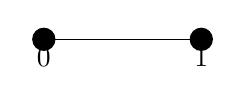
\begin{tikzpicture}[scale=2]
    \draw (0,0) -- (1,0);
    \foreach \x in {0,1}
        \filldraw (\x,0) circle (2pt) node[below] {$\x$};
    \end{tikzpicture}
    \hfill
    % B2 Visualization
    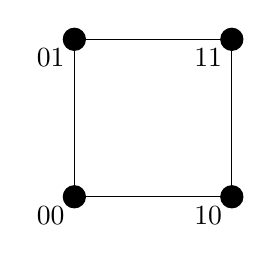
\begin{tikzpicture}[scale=2]
    \draw (0,0) rectangle (1,1);
    \foreach \x in {0,1}
      \foreach \y in {0,1}
        \filldraw (\x,\y) circle (2pt) node[below left] {$\x\y$};
    \end{tikzpicture}
    \hfill
    % B3 Visualization
    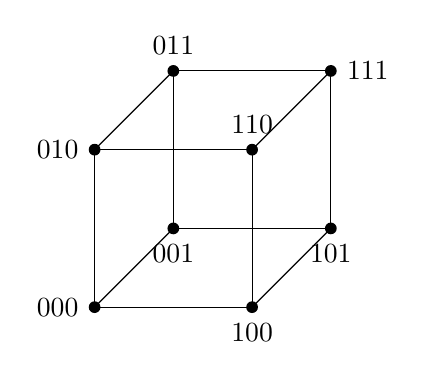
\begin{tikzpicture}[scale=2]
        % Define style for the nodes
        \tikzstyle{vertex}=[circle,fill,inner sep=1.5pt]
        
        % Draw the back square
        \draw (0,0) node[vertex,label=left:{000}] {} -- (0,1) node[vertex,label=left:{010}] {} -- (1,1) node[vertex,label=above:{110}] {} -- (1,0) node[vertex,label=below:{100}] {} -- cycle;
        
        % Draw the front square
        \draw (0.5,0.5) node[vertex,label=below:{001}] {} -- (0.5,1.5) node[vertex,label=above:{011}] {} -- (1.5,1.5) node[vertex,label=right:{111}] {} -- (1.5,0.5) node[vertex,label=below:{101}] {} -- cycle;
        
        % Connect the vertices
        \draw (0,0) -- (0.5,0.5);
        \draw (0,1) -- (0.5,1.5);
        \draw (1,1) -- (1.5,1.5);
        \draw (1,0) -- (1.5,0.5);
        \end{tikzpicture}
        \caption{Visualization of Boolean Domain}
\end{figure}

    \section{Predicates and Quantifiers}
We have covered the knowledge that allows us to work around with boolean variables and logical operators and simplify logical circuits accordingly. However, the most interesting part of logic is not yet mentioned. Before that, we need to work out predicate and quantifiers that will be used to adding details to our statements so that they can be more precise and also avoid ambiguous interpretations. This part of logic is more accessible, and less boring, because we can relate all these to natural language rather than circuits.

\subsection{Predicate}
When you see the word "predicate", you may feel like you are having a primary school English class, where you learn basic grammars. Well, the predicate in mathematics is indeed pretty much the same as what we see the the English language. The definition we all have known is listed below.
\begin{definition}[Predicate]
    Predicate is the part of a sentence containing a verb that makes a statement about the subject of the verb, such as "went home" in John went home. In mathematics, predicate is regarded as a \textit{Boolean function}. Usually, a predicate is denoted by $P$ by convention, but preferably, it can be anything you want, or even a word. Like what we do for writing a function, we write the inputs, or we say the objects involved in the statement in a pair of parenthesis (can be any number). 
\end{definition}

\begin{example}
    We can define a predicate $P$, where for $P(x)$, $x$ is the first name of someone, means that $x$ begins with letter "E". So $P(\text{Eric})\equiv 1$, and $P(\text{Alex})\equiv 0$.
\end{example}

\begin{example}
    We define a predicate $Less(x, y)$ on integers, meaning that $x < y$. So we have $Less(2, 3) \equiv 1$ and $Less(3, 2) \equiv 0$. 
\end{example}

\begin{remark}
    Notice that, sometimes a predicate is defined without specifying the type of objects that involved, so whether it is valid depends on the arguments. 
\end{remark}

In Computer Science, an important application of predicate is determining program correctness by checking \textbf{preconditions} and \textbf{post conditions}.

\begin{definition}[Precondition]
     A precondition is a condition or set of conditions that must be true before the execution of a program or a procedure. Preconditions are used to specify the requirements or constraints on the inputs for the procedure to function correctly.
\end{definition}

\begin{definition}[Postcondition]
    A postcondition is a condition or set of conditions that must be true after the execution of a program or a procedure, assuming that the preconditions were true. Postconditions specify the expected state of the outputs and the system once the procedure has completed.
\end{definition}
Consider the following example related to predicate logic. 

\begin{example}
    Suppose we have a procedure that takes an integer \( n \) and returns the factorial of \( n \). The precondition for this procedure is that \( n \) must be a non-negative integer. The postcondition is that the returned value must be equal to the product of all positive integers up to \( n \).

Formally, let \( P(n) \) denote the predicate "the input \( n \) is a non-negative integer," and let \( Q(n, f(n)) \) denote the predicate "the output \( f(n) \) is the factorial of \( n \)." We can express the precondition and postcondition as follows:

\begin{itemize}
    \item \textbf{Precondition:} \( P(n) \equiv (n \geq 0) \)
    \item \textbf{Postcondition:} \( Q(n, f(n)) \equiv (f(n) = n!) \)
\end{itemize}

If the precondition \( P(n) \) holds, then after executing the procedure, the postcondition \( Q(n, f(n)) \) must hold, ensuring that the procedure correctly computes the factorial of \( n \).
\end{example}

\subsection{Quantifier}
With predicate, we can specify statements for different scenarios, yet we can add more constraints to our statements. In English, we always use pronouns with some or any/every as in "someone", "anyone", or "everyone". There is no lack of such usage when we are speaking natural language. Don't take quantifier as something complex, what we do in math is only formalize and symbolize such meaning or usage in natural language so that they are more reliable for mathematical reasoning.

\begin{definition}[Quantifier]

Quantifiers are symbols used in logic to express the extent to which a predicate is true over a range of elements. The two most common quantifiers are the universal quantifier and the existential quantifier.

\begin{description}
    \item[Universal Quantifier] The universal quantifier, denoted by $\forall$, asserts that a predicate is true for all elements in a given domain. It is read as "for all" or "for every". Formally, $\forall x \in D, P(x)$ means that for every element $x$ in the domain $D$, the predicate $P(x)$ holds true.
    \item[Existential Quantifier] The existential quantifier, denoted by $\exists$, asserts that there exists at least one element in the domain for which the predicate is true. It is read as "there exists" or "for some". Formally, $\exists x \in D \text{ such that } P(x)$ means that there is at least one element $x$ in the domain $D$ for which the predicate $P(x)$ holds true.
\end{description}
\end{definition}
\begin{remark}
    We also have a quantifier called uniqueness quantifier which uses the same notation as for existential quantifier. The only difference is that we write $\exists_x$ to express that there are exactly $x$ cases that the interpretation is true.
\end{remark}
\begin{example}
\begin{equation*}
    \forall x \in \mathbb{R}, x^2 \geq 0
\end{equation*}
This statement asserts that for all real numbers $x$, the square of $x$ is greater than or equal to zero.
\end{example}
\begin{example}
\begin{equation*}
    \exists x \in \mathbb{R} \text{ such that } x^2 = 4
\end{equation*}
This statement asserts that there exists a real number $x$ such that the square of $x$ is equal to 4. Indeed, $x = 2$ or $x = -2$ satisfy this condition.
\end{example}

Actually, quantifiers can be written as logical operations of predicates. Suppose we define $P(x)$ on \seq{x}{1}{k}. Then we have
\[\forall x P(x) \equiv \bigwedge_{i=1}^{k} P(x_i) = P(x_1)\land P(x_2)\land \cdots \land P(x_k).\]

Similarly, we have 
\[\exists x P(x) \equiv \bigvee_{i=1}^{k} P(x_i) = P(x_1)\lor P(x_2)\lor \cdots \lor P(x_k).\]


As a shorthand, we can write the domain or condition to the variables in the quantifier and write the predicate in math expression.
\begin{example}
    Every negative number are positive after square can be written as
    \[\forall x < 0 (x^2>0).\]
    Where the predicate it put inside parenthesis.
\end{example}

Sometimes, or in most cases, a single quantifier is not enough to express the statement we want to present. In that case, we need to use multiple quantifiers. Consider the statement "For all natural number, there exists natural number that is two times of them." We can write it as
\[\forall x\in \N\exists y \in \N(y=2x).\]

This is obviously true, however, if we write
\[\exists  x\in \N\forall y \in \N(y=2x).\]
We can find that it does not hold, since there is no such $x$ to be half of any $y$.

Another important aspect of quantifier when we deal with predicate with multiple variables is bounded variable.
\begin{definition}[Bounded Variable]
    A variable \( x \) is said to be \textbf{bounded} by a quantifier in a logical formula if it appears within the scope of a quantifier such as \(\forall\) (for all) or \(\exists\) (there exists), else we call it a free variable. 

The scope of the quantifier includes the part of the formula where the variable is explicitly governed by the quantifier.
\end{definition}

\begin{example}
Consider the logical statement:
\[ \forall x \in \mathbb{N} \, \exists y \in \mathbb{N} \, (x < y) \]
In this statement:
\begin{itemize}
    \item The variable \( x \) is bounded by the universal quantifier \(\forall x\).
    \item The variable \( y \) is bounded by the existential quantifier \(\exists y\).
\end{itemize}
Both \( x \) and \( y \) are bounded variables within their respective scopes. Outside the scope of these quantifiers, the variables would be considered free.
\end{example}

Quantifiers can also be joined with logical operators, and here we provide proof to the only logical equivalence on simple quantifiers.
\begin{theorem}
\(\forall x (P(x) \land Q(x))\) and \(\forall x P(x) \land \forall x Q(x)\) are logically equivalent.
\end{theorem}

\begin{proof}
To show that these statements are logically equivalent, we must show that they always take the same truth value, no matter what the predicates \(P\) and \(Q\) are, and no matter which domain of discourse is used. Suppose we have particular predicates \(P\) and \(Q\), with a common domain. We can show that \(\forall x (P(x) \land Q(x))\) and \(\forall x P(x) \land \forall x Q(x)\) are logically equivalent by doing two things. First, we show that if \(\forall x (P(x) \land Q(x))\) is true, then \(\forall x P(x) \land \forall x Q(x)\) is true. Second, we show that if \(\forall x P(x) \land \forall x Q(x)\) is true, then \(\forall x (P(x) \land Q(x))\) is true.

So, suppose that \(\forall x (P(x) \land Q(x))\) is true. This means that if \(a\) is in the domain, then \(P(a) \land Q(a)\) is true. Hence, \(P(a)\) is true and \(Q(a)\) is true. Because \(P(a)\) is true and \(Q(a)\) is true for every element \(a\) in the domain, we can conclude that \(\forall x P(x)\) and \(\forall x Q(x)\) are both true. This means that \(\forall x P(x) \land \forall x Q(x)\) is true.

Next, suppose that \(\forall x P(x) \land \forall x Q(x)\) is true. It follows that \(\forall x P(x)\) is true and \(\forall x Q(x)\) is true. Hence, if \(a\) is in the domain, then \(P(a)\) is true and \(Q(a)\) is true (because \(P(x)\) and \(Q(x)\) are both true for all elements in the domain, there is no conflict using the same value of \(a\) here). It follows that for all \(a\), \(P(a) \land Q(a)\) is true. It follows that \(\forall x (P(x) \land Q(x))\) is true. We can now conclude that
\[
\forall x (P(x) \land Q(x)) \equiv \forall x P(x) \land \forall x Q(x).
\]
\end{proof}

Then, how can we negate a quantifier?

Consider this statement: Everyone in this room likes banana.
We use $P(x)$ to show that the individual $x$ likes banana.
Then we have \[\forall x P(x).\]

We can negate in natural language that: someone in this room dislikes banana, which can be written as
\[\exists x\neg P(x).\]
You may have already found the pattern, to negate the whole expression, we replace all universal quantifiers to existential quantifiers and vice versa, finally we negate the predicate. We call these rules De Morgan's law for quantifiers.

\begin{table}[H]
\centering
\caption{De Morgan's law for quantifiers}
\begin{tabular}{|c|c|c|c|}
\hline
\textbf{Negation} & \textbf{Equivalence} & \textbf{When True?} & \textbf{When False?} \\
\hline
$\neg \exists x P(x)$ & $\forall x \neg P(x)$ & For every $x$, $P(x)$ is false. & Exists $x$ for which $P(x)$ is true. \\
\hline
$\neg \forall x P(x)$ & $\exists x \neg P(x)$ & Exists $x$ for which $P(x)$ is false. & $P(x)$ is true for every $x$. \\
\hline
\end{tabular}
\end{table}

\subsection{Nested Quantifier}



    \section{Inference and Deduction}